\section{Modeling}
\label{sec:modeling}

In this section, we will present the modeling of the ADC and DAC. The developed code is present in the appendix \ref{apendice:github}.

\subsection{DAC}

With equation \ref{eq:DeltaVx}, the model only needs to store the last value of $V_x$ and most importantly, the variation on the output node caused by each bit, can be previously calculated and simply accessed, avoiding redundant computing.  

Hence, the first step in modeling the DAC is creating a function that precompute the DAC weights. For the Ideal values, each weight is represented in Table \ref{tab:DACWeights}.


\begin{table}[h]

    \centering
    \caption{DAC Bit weights.}
    \begin{tabularx}{\textwidth}{
        >{\centering\arraybackslash}X 
        >{\centering\arraybackslash}X 
        >{\centering\arraybackslash}X 
        >{\centering\arraybackslash}X 
        >{\centering\arraybackslash}X 
        >{\centering\arraybackslash}X 
        >{\centering\arraybackslash}X 
        >{\centering\arraybackslash}X 
        >{\centering\arraybackslash}X 
        >{\centering\arraybackslash}X 
        >{\centering\arraybackslash}X 
        >{\centering\arraybackslash}X 
        }
        \toprule
        \textbf{Bit Value}  & \textbf{$B_{10}$}& \textbf{$B_{9}$}& \textbf{$B_{8}$}& \textbf{$B_{7}$}& \textbf{$B_{6}$}& \textbf{$B_{5}$}& \textbf{$B_{4}$}& \textbf{$B_{3}$}& \textbf{$B_{2}$}& \textbf{$B_{1}$}& \textbf{$B_{0}$}\\
        \midrule
        $1$ & 250     & 125     & 62.5    & 31.25   & 15.63  & 7.81 & 7.81 & 3.91& 1.95& 0.98& 0.488  \\
        \midrule
        $0$ & -250  & -125   & -62.5     & -31.3    & -15.6   & -7.8 & 0 & 0 & 0 & 0 & 0  \\    
        \bottomrule
    \end{tabularx}
    \label{tab:DACWeights}
\end{table}

In this step it is important to remember that the circuit is differential, otherwise the DAC will not work for all bits, because the hybrid capacitors will have a positive change in one node and negative at the other, Table \ref{tab:DACWeights} shows exactly that. 

Now, with the weights computed the DAC output is show in Figure \ref{fig:DAC_TF}.

\begin{equation}
    V_{DAC} = \sum_{i}^{\text{code}}\Delta V_{xp}(b_i)- \Delta V_{xn}(\neg b_i)
    \label{eq:VDAC}
\end{equation}

\begin{figure}[h]
    \centering

    \begin{subfigure}[b]{0.9\textwidth}
        \centering
        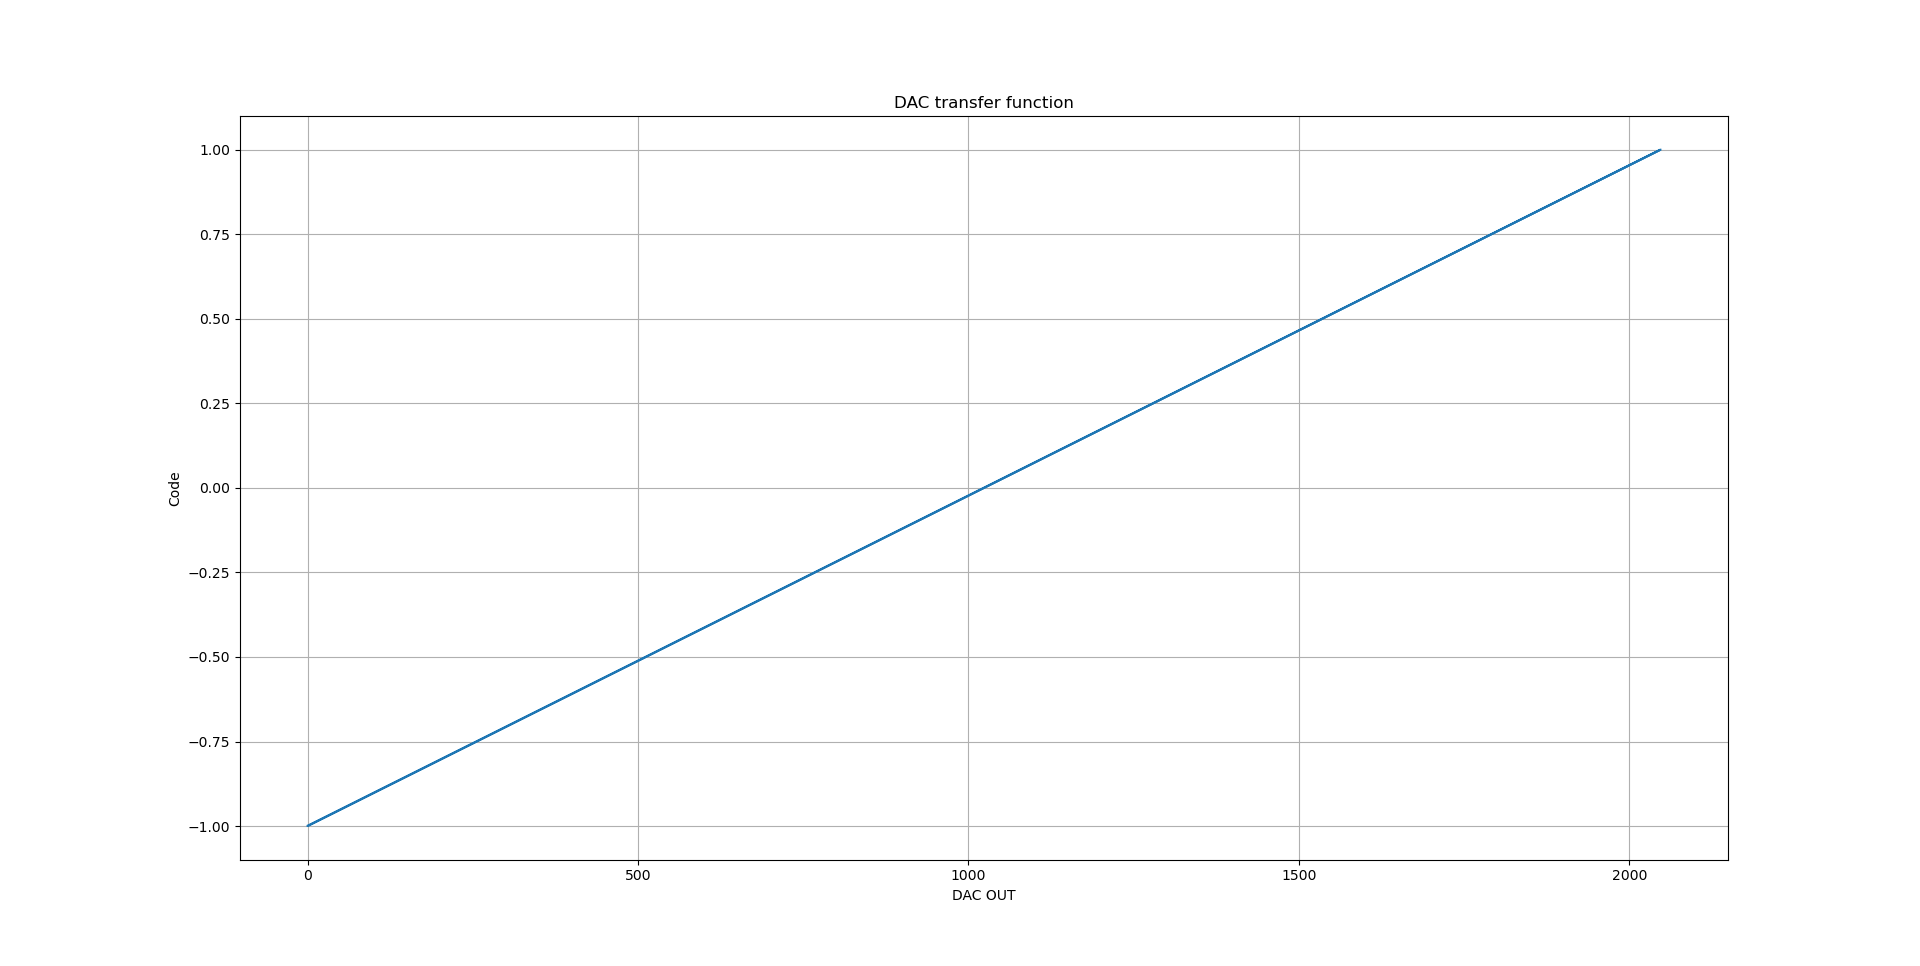
\includegraphics[width=\textwidth]{Images/DAC_TransFunc_ideal.png}
        \caption{Ideal DAC Transfer Function.}
        \label{fig:DAC_TF}
    \end{subfigure}%

    \begin{subfigure}[b]{0.5\textwidth}
        \centering
        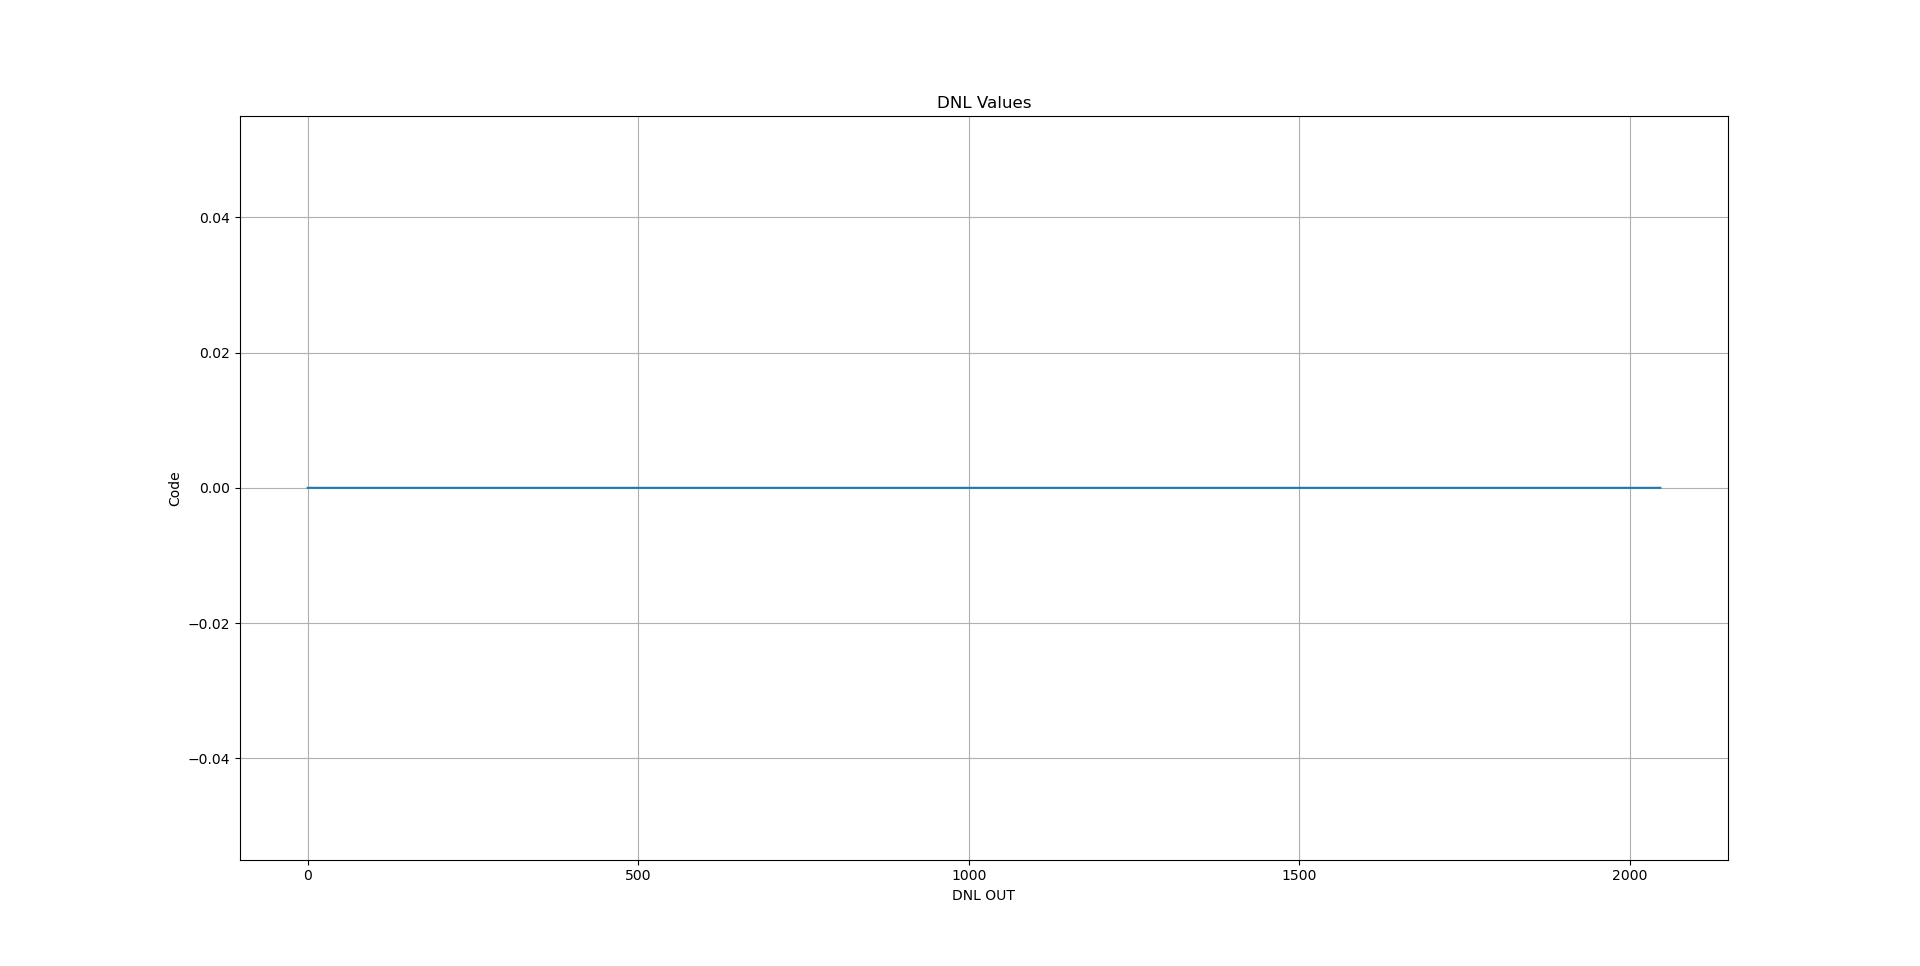
\includegraphics[width=\textwidth]{Images/DAC_DNL_ideal.png}
        \caption{Ideal DAC DNL.}
        \label{fig:DAC_DNL}
    \end{subfigure}%
    \begin{subfigure}[b]{0.5\textwidth}
        \centering
        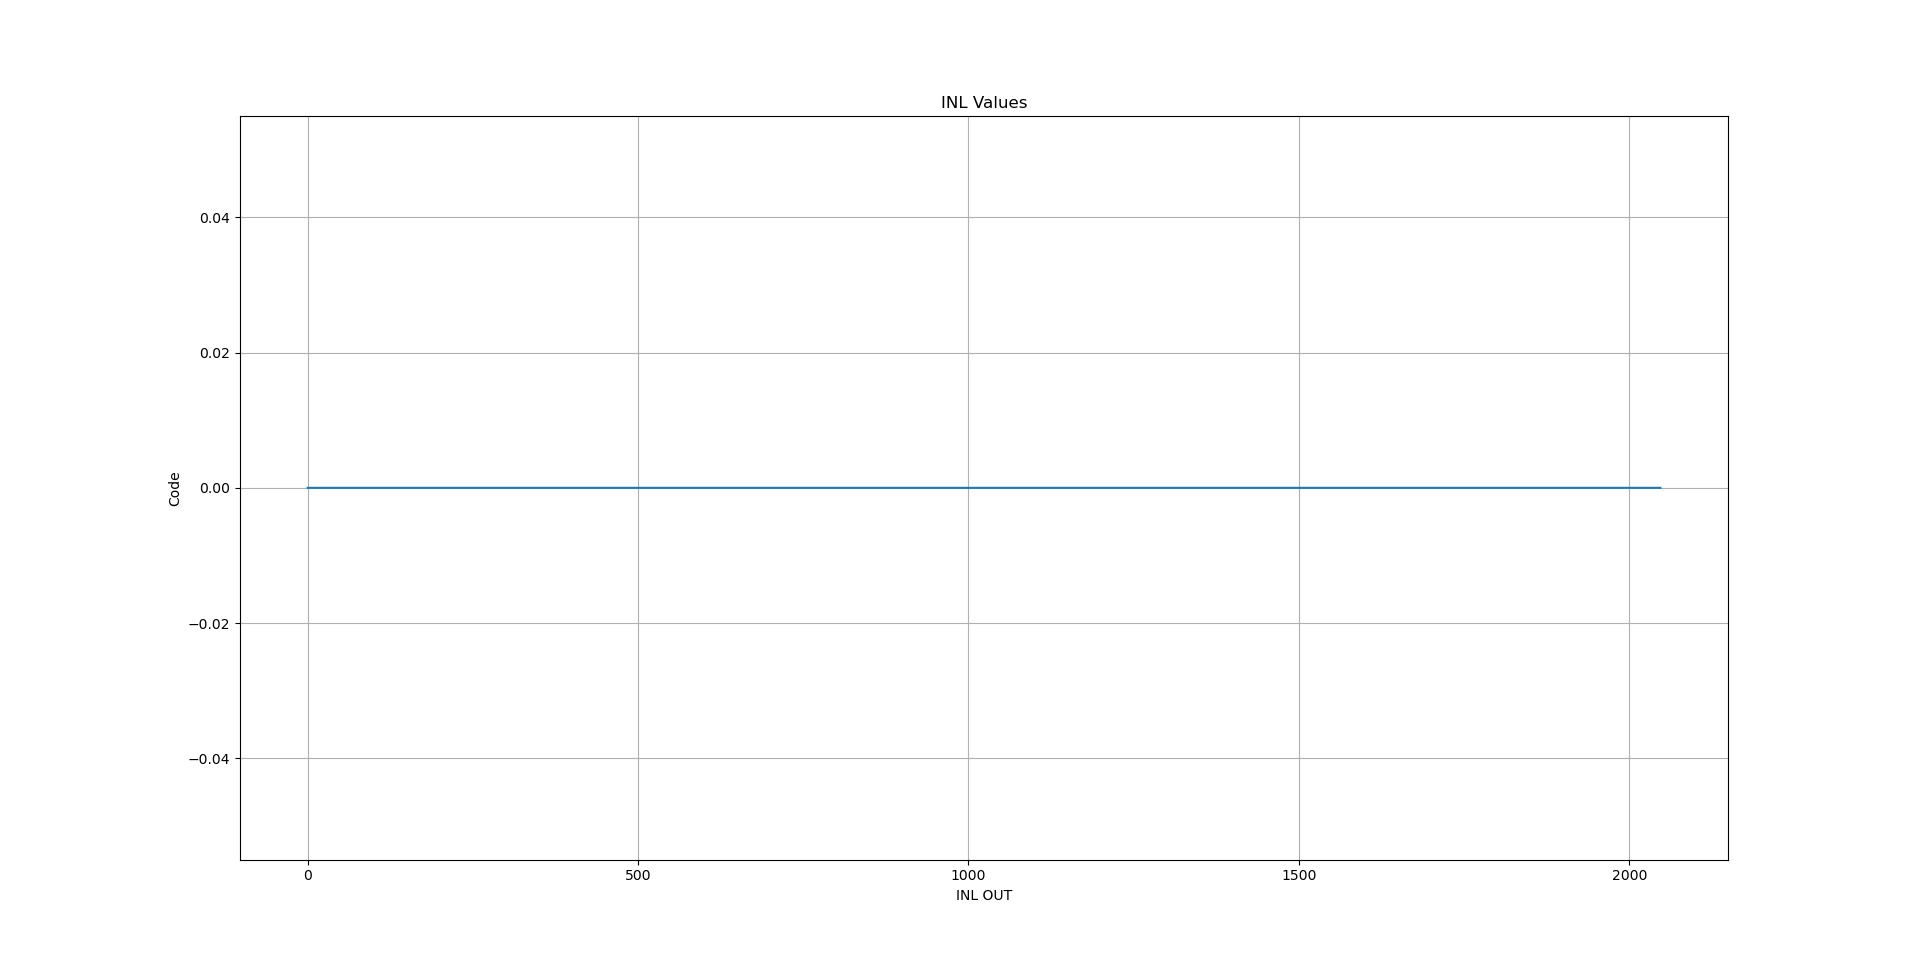
\includegraphics[width=\textwidth]{Images/DAC_INL_ideal.png}
        \caption{Ideal DAC INL.}
        \label{fig:DAC_INL}
    \end{subfigure}

    \caption{DAC validation.}
    \label{fig:IdealDAC}
\end{figure}

Figure \ref{fig:IdealDAC} was obtained by sweeping all codes and computing the INL and DNL. For this test $V_{ref} = 2$ and the ideal values for the capacitors were considered. This works as expected with a linear transfer function, Figure \ref{fig:DAC_TF}, and always 0 DNL and INL values, Figures \ref{fig:DAC_DNL} and \ref{fig:DAC_INL}.

\subsection{ADC}

The first step in the ADC modeling is to make a function that mimics the ADC's process, by plotting the $V_{xp}$ and $V_{xn}$ evolution after each iteration, i.e., after each comparison of the comparator of the ADC, and the contribution of the DAC for $V_{xp}$ and $V_{xn}$. With this function, the debug and validation of the ADC is easier.

\begin{comment}
    
    vip   = vin/2 +1
    vin   = -vin/2 +1
    ind   = n_bits_dac  
    b_aux = vip > vin
    res   = bit_masks[n_bits_dac]*b_aux

    vip_arr = [ float() for _ in range(n_bits+1) ]
    vin_arr = [ float() for _ in range(n_bits+1) ]

    vip_arr[0] = vip
    vin_arr[0] = vin

    j = 1
    for  i in range(n_bits_dac-1,-1,-1):
        vip   += dac_weights_plus[i][np.uint8(not(b_aux))]
        vin   += dac_weights_minus[i][np.uint8(b_aux)]
        vip_arr[j] = vip
        vin_arr[j] = vin
        j     += 1
        b_aux  = vip + Voffset > vin        
        ind   -= 1
        res   += bit_masks[i]*b_aux
    
\end{comment}

\begin{figure}[h]

    \centering
    \includegraphics*[width=0.9\textwidth]{Images/Vxp_Vxn_evolution_1V_input.png}
    \caption{$V_{xp}$ and $V_{xn}$ evolution $V_{in} = 1$.}

    \label{fig:VxpVxnEvo}
\end{figure}

As demonstrated in Figure \ref{fig:VxpVxnEvo}, the values of $V_{xp}$ and $V_{xn}$ tend to the value of the common-mode voltage, equal to $\frac{V_r}{2}$, this means that the central value between both differential inputs remains the same for every iteration, this is the result of the hybrid capacitors configuration present in the higher values capacitors, mentioned before. Although this architecture does not exist for the last iterations, the central value does not differ much from the desired value, since the output of the DAC for the least significant bits is much smaller than the one for the most significant bits, therefore the variation this central value can be negligible.

This maintenance of the central value is what guarantees that the differential value between $V_{xp}$ and $V_{xn}$ represents the original input value of $V_{in}$, confirming the ADC model presented is working properly.

Now having confirmed the ADC functionality a simpler function was developed and explain in  the flowchart depicted in Figure \ref{fig:ADCFlowChart}, since there is no need to keep the values of both nodes.
The first simplification made was to the circuit's differential nature, the comparator's output, with $V_{Offset}$ effect, is shown in Equation \ref{eq:CompOut}.

\begin{equation}
    V_{xp} + V_{offset} > V_{xn} \Leftrightarrow \overbrace{( V_{xp} - V_{xn} )}^{V_x} > V_{offset} 
    \label{eq:CompOut}
\end{equation}

\begin{figure}[h]

    \centering
    \includegraphics*[width=0.8\textwidth]{Images/ADCPythonFlowChart.png}
    \caption{ADC Python function FLowchart.}

    \label{fig:ADCFlowChart}
\end{figure}

\subsubsection{Code Validation}

Now in order to get the ADC characteristic curve, a ramp input signal was generated and then the transition points were collected, giving a tuple output, $\text{ADC Transitions} \longrightarrow ( D_{out}, V_{in} ) $, were $D_{out}$ is the digital output and $V_{in}$ is the analog input that first changed the code to $D_{out}$, the curve is shown in Figure \ref{fig:ADC_TF_Ideal}.

For testing a ramp with 1000 points per $V_{LSB}$ was used, this is way more than what is needed, for the following simulations 50 points per $V_{LSB}$ was used.


\begin{figure}[H]
    \centering

    \begin{subfigure}[b]{0.9\textwidth}
        \centering
        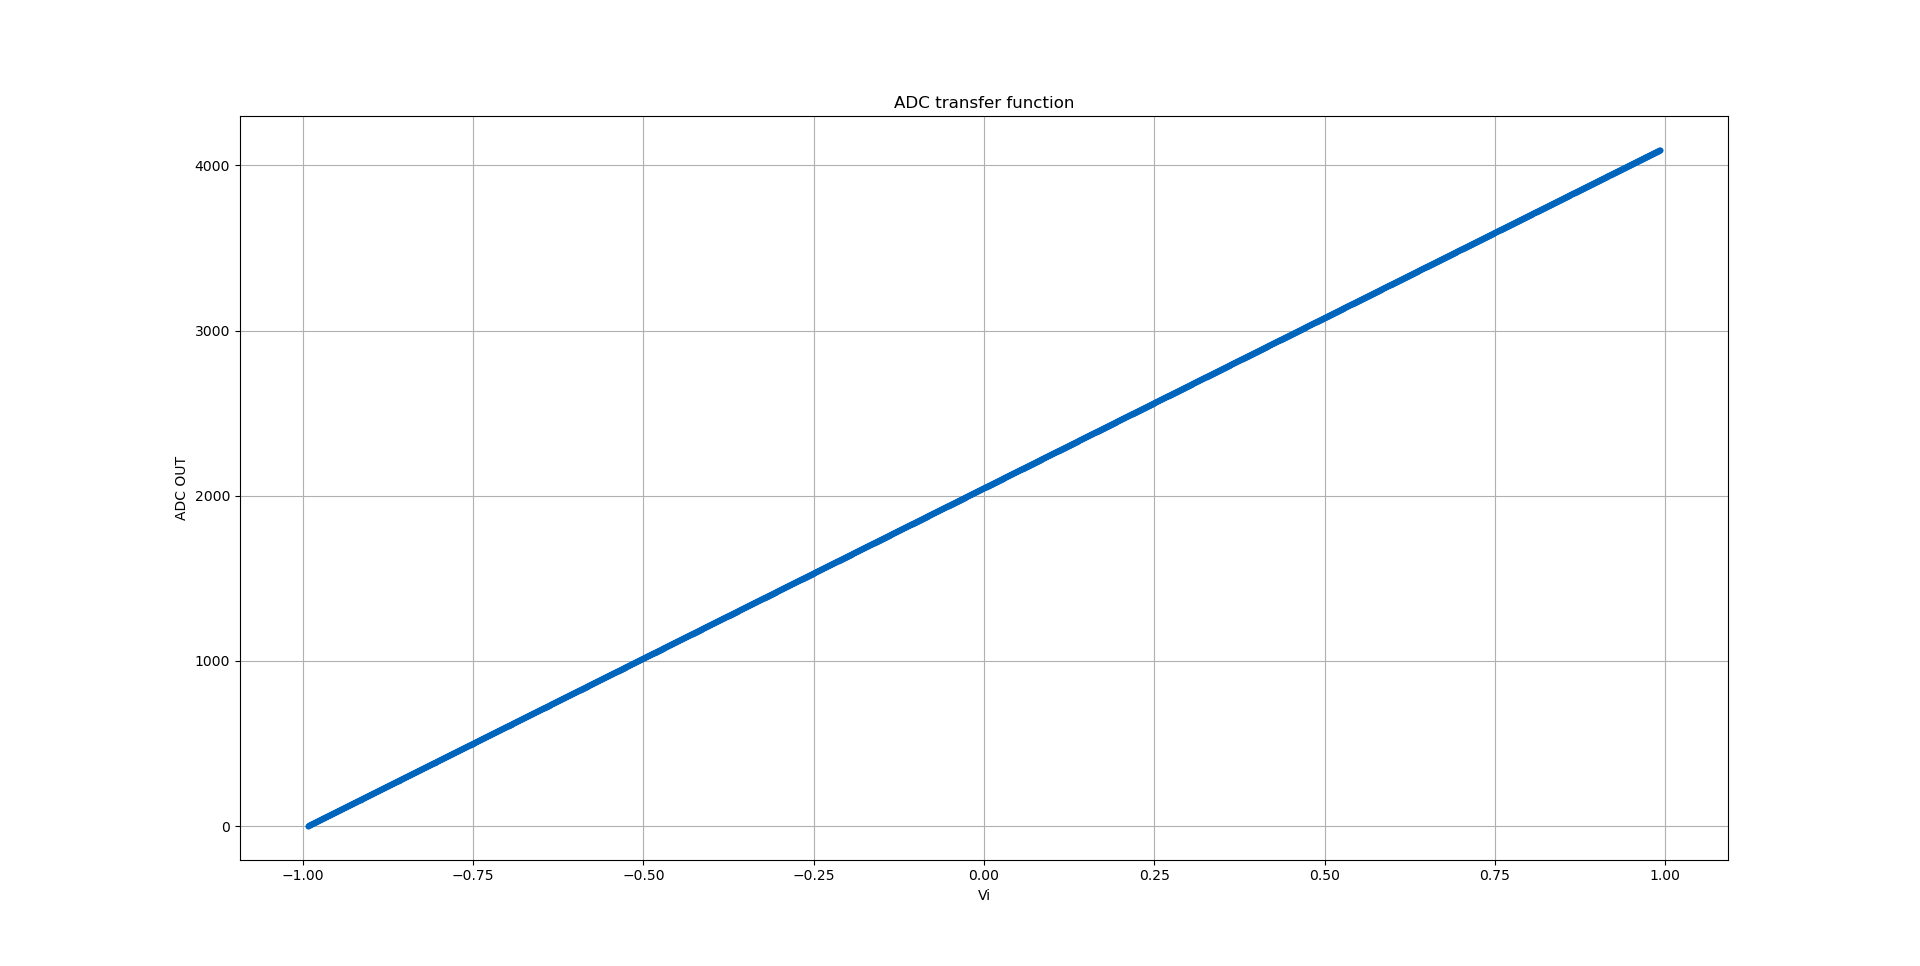
\includegraphics[width=\textwidth]{Images/ADC_TransFunc_Ideal.png}
        \caption{Ideal ADC Transfer Function.}
        \label{fig:ADC_TF_Ideal}
    \end{subfigure}%

    \begin{subfigure}[b]{0.5\textwidth}
        \centering
        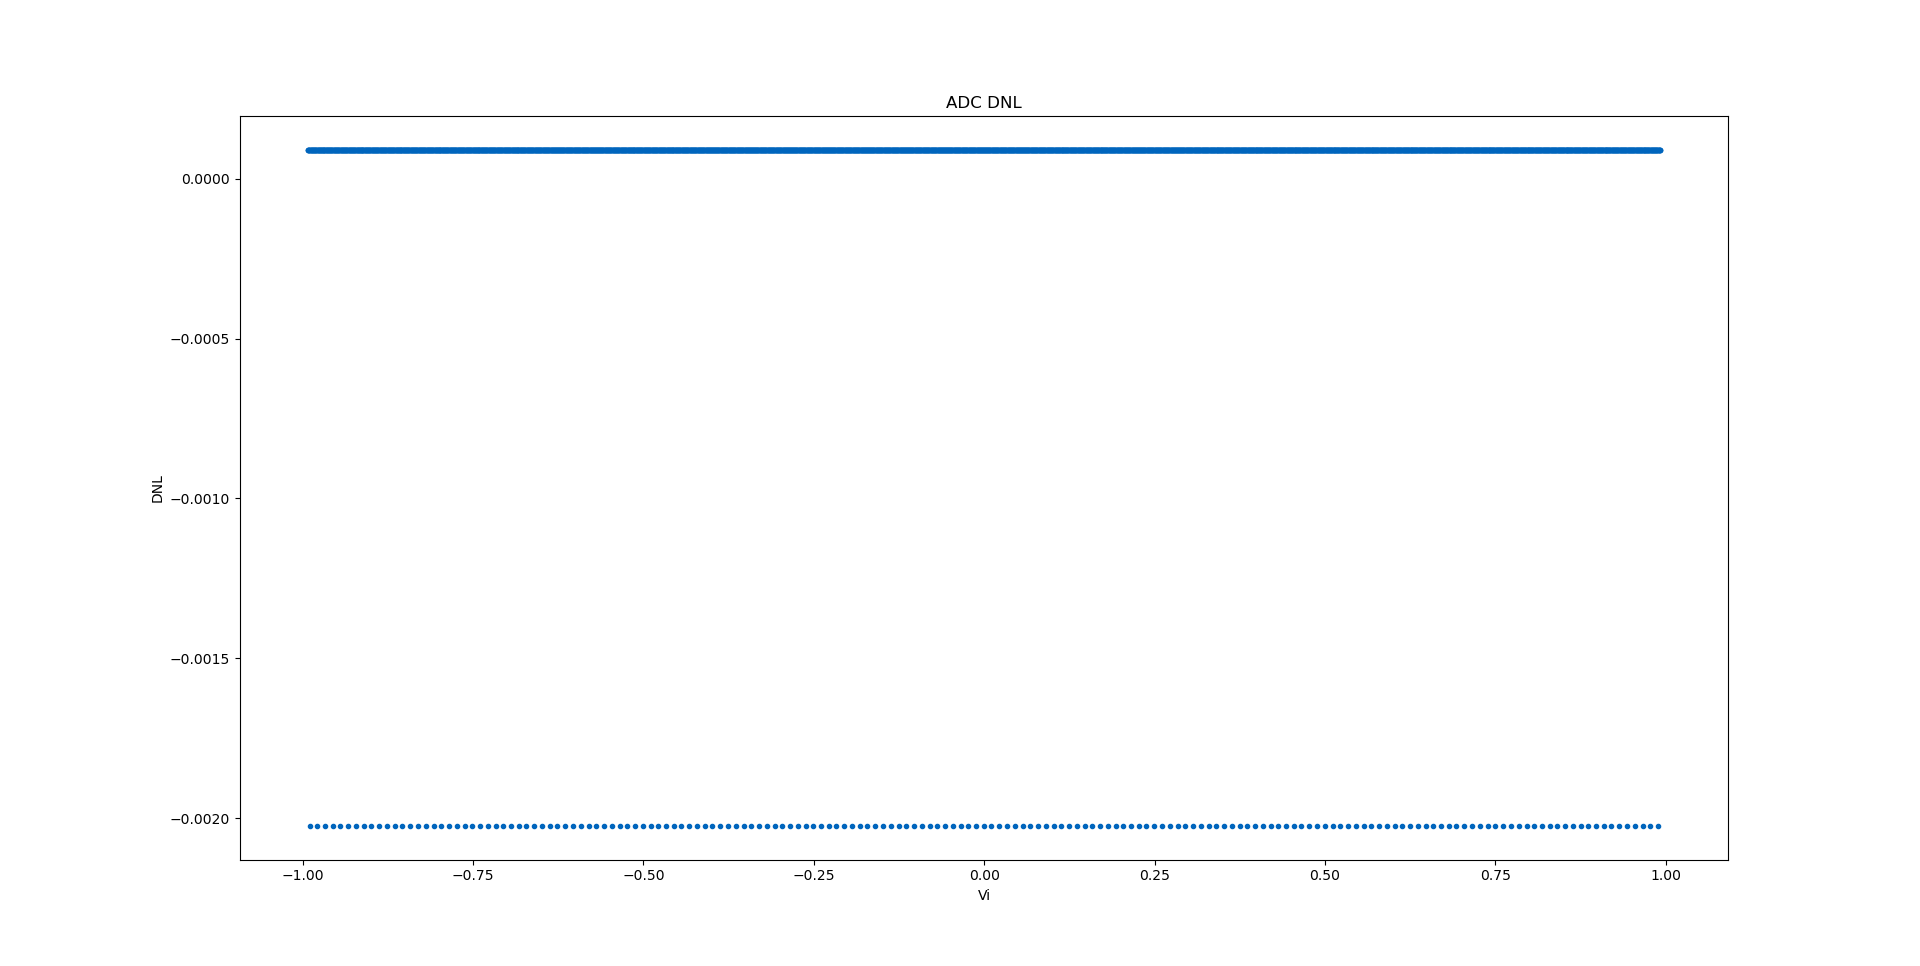
\includegraphics[width=\textwidth]{Images/DNL_Ideal.png}
        \caption{Ideal ADC DNL.}
        \label{fig:ADC_DNL_Ideal}
    \end{subfigure}%
    \begin{subfigure}[b]{0.5\textwidth}
        \centering
        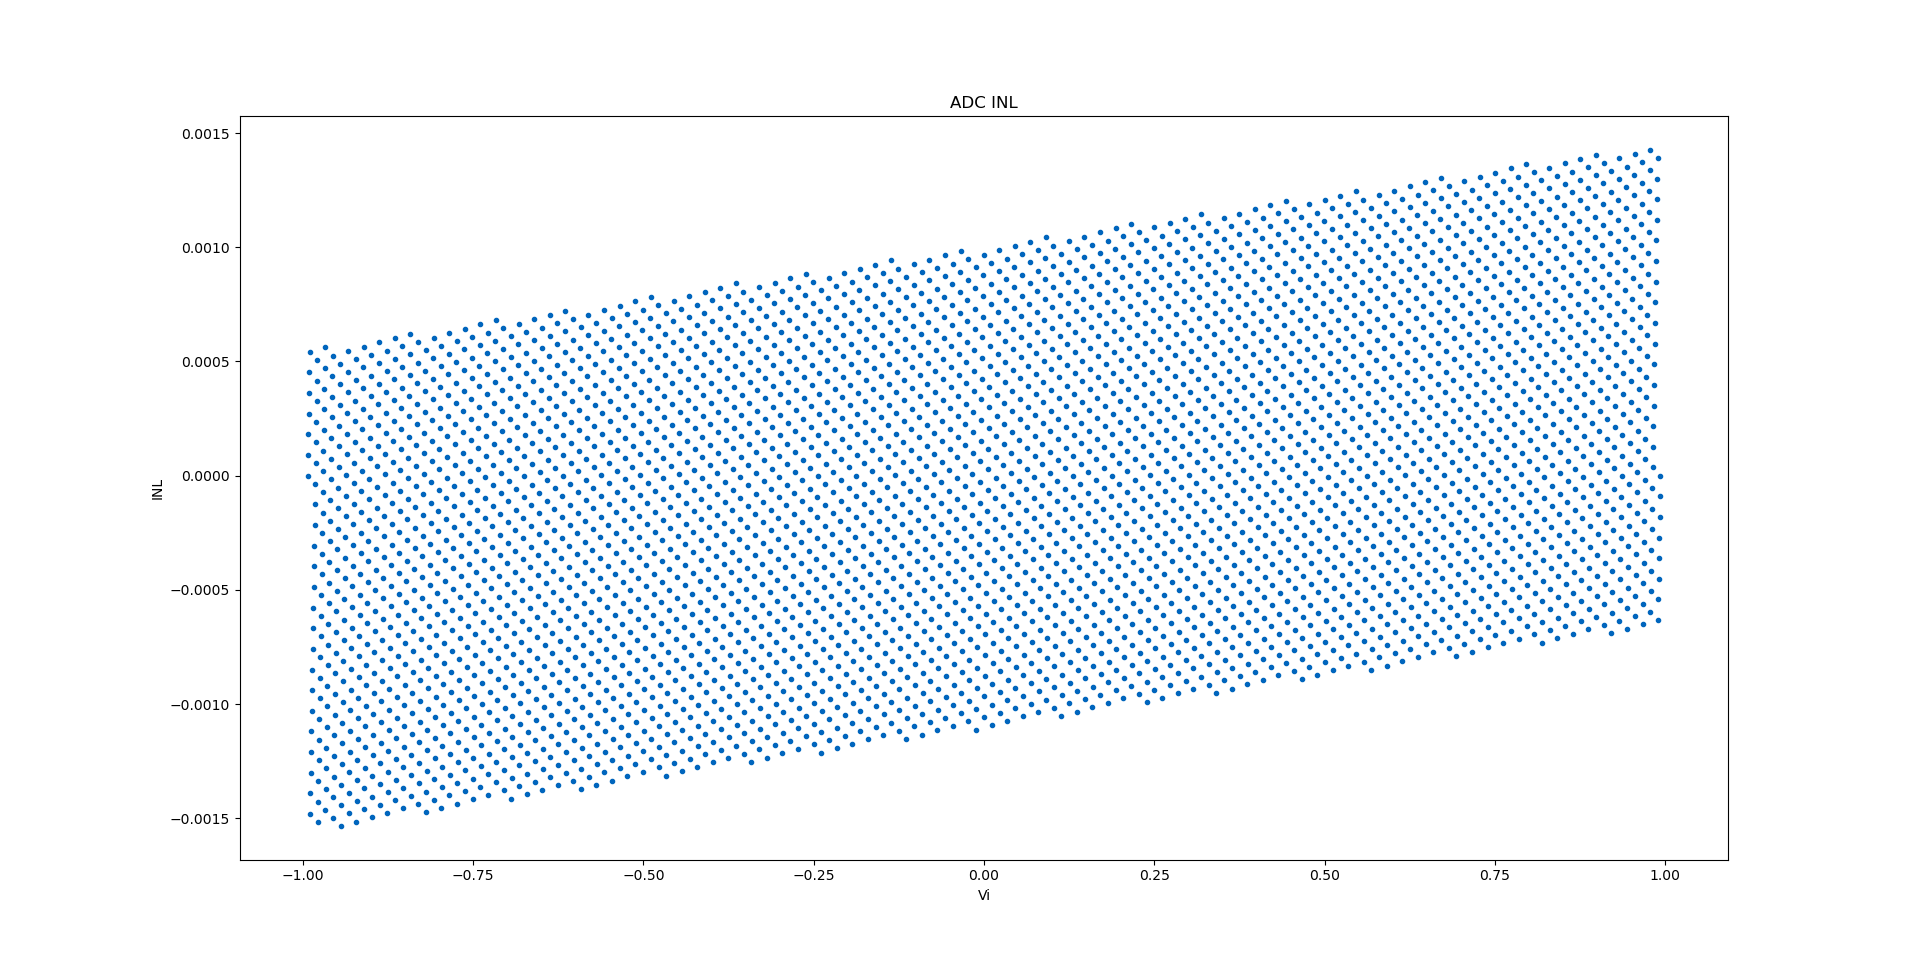
\includegraphics[width=\textwidth]{Images/INL_Ideal.png}
        \caption{Ideal ADC INL.}
        \label{fig:ADC_INL_Ideal}
    \end{subfigure}

    \caption{ADC validation}
    \label{fig:IdealADC}
\end{figure}

The values of INL and DNL for the ideal ADC, unlike the values for the DAC, were not equal to $0$ LSB, since the input for the ADC was not a real continuos signal, only an array of point, mimicking this analog input, resulting in a lack of precision, this result is shown in Firures \ref{fig:ADC_DNL_Ideal} and \ref{fig:ADC_INL_Ideal}.

\subsection{Spectral Analysing}

\begin{equation}
    SNDR = 10 \log_{10} \left( \frac{P_{\text{signal}}}{P_{\text{noise}} + P_{\text{distortion}}} \right)  \quad \text{(in dB)} \textsuperscript{\cite{analogIntegratedCircBook}}
    \label{eq:SNDR}
\end{equation}

In order to calculate $SNDR$ an input signal was created,$v_{in}$ , in this case a sine wave with frequency $\SI{1}{\hertz}$. This signal is sampled by the ADC and the output is stored, $v_{out}$.

Now the Fourier Transform is computed for both.

\begin{equation}
    \begin{split}
        \mathcal{F}\{v_{in}(t)\} &\rightarrow V_{IN}(f)\\
        \mathcal{F}\{v_{out}(t)\} &\rightarrow V_{OUT}(f)\\
    \end{split}
    \label{eq:fourier}
\end{equation}

Therefore $N(f) = V_{IN} - V_{OUT}$ where $N(f)$ is the noise spectrum, the graphical representation of $v_{in}$,$V_{IN}$, $V_{OUT}$ and $N(f)$ is depicted in Figure \ref{fig:Noise Ideal}. Hence, the noise power is given by Equation \ref{eq:NoisePower}.

\begin{equation}
    P_{noise} = \int_{0}^{+\infty}|N(f)|^2 
    \label{eq:NoisePower}
\end{equation}

\begin{figure}[h]
    \centering

    \begin{subfigure}[b]{0.4\textwidth}
        \centering
        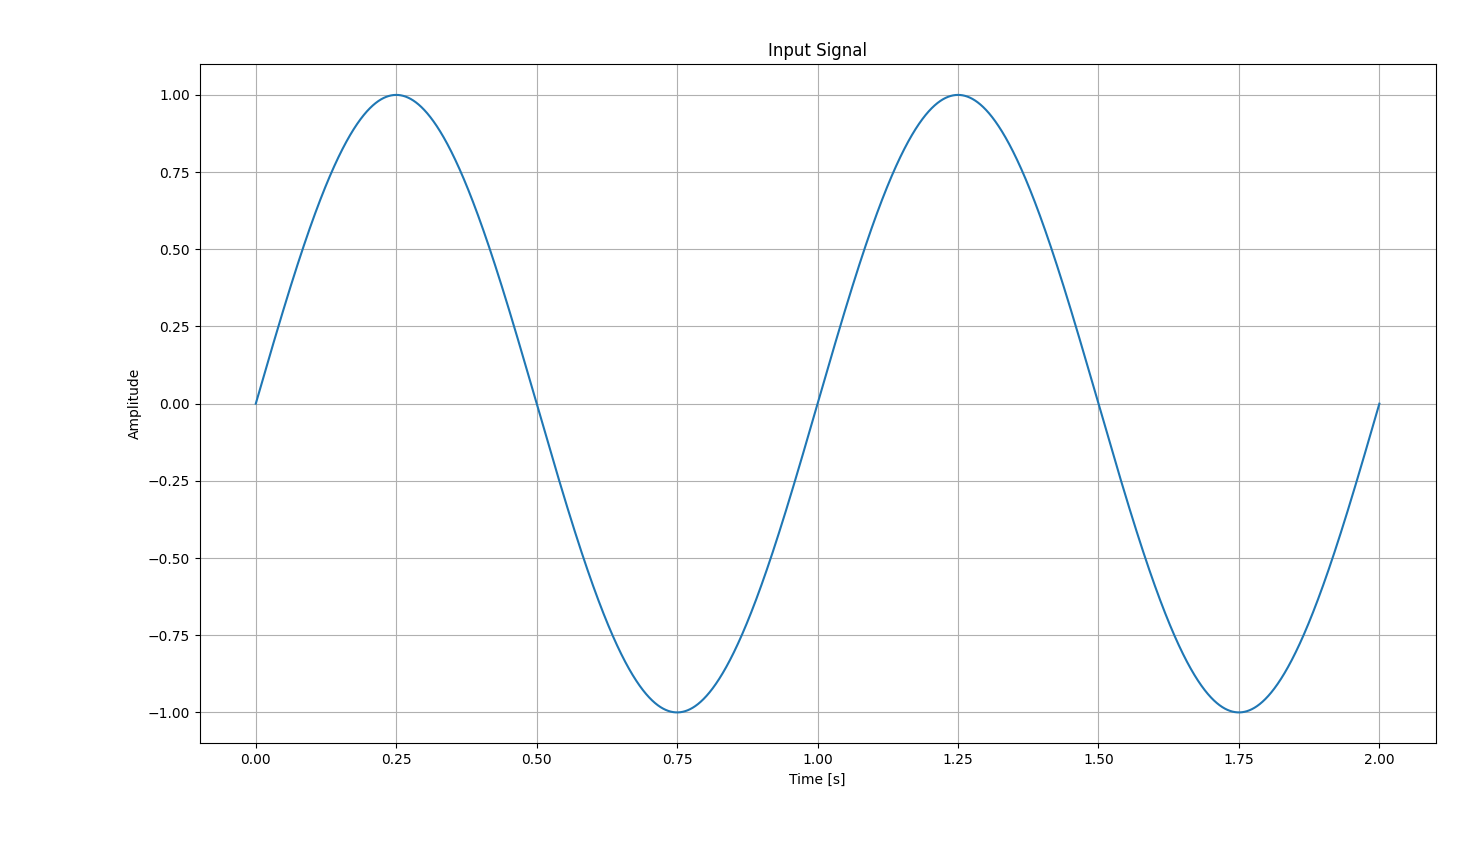
\includegraphics[width=\textwidth]{Images/Vin_tempo_ideal.png}
        \caption{$v_{in}(t)$ - Input signal.}
        \label{fig:Vin_tempo_ideal}
    \end{subfigure}%
    \begin{subfigure}[b]{0.4\textwidth}
        \centering
        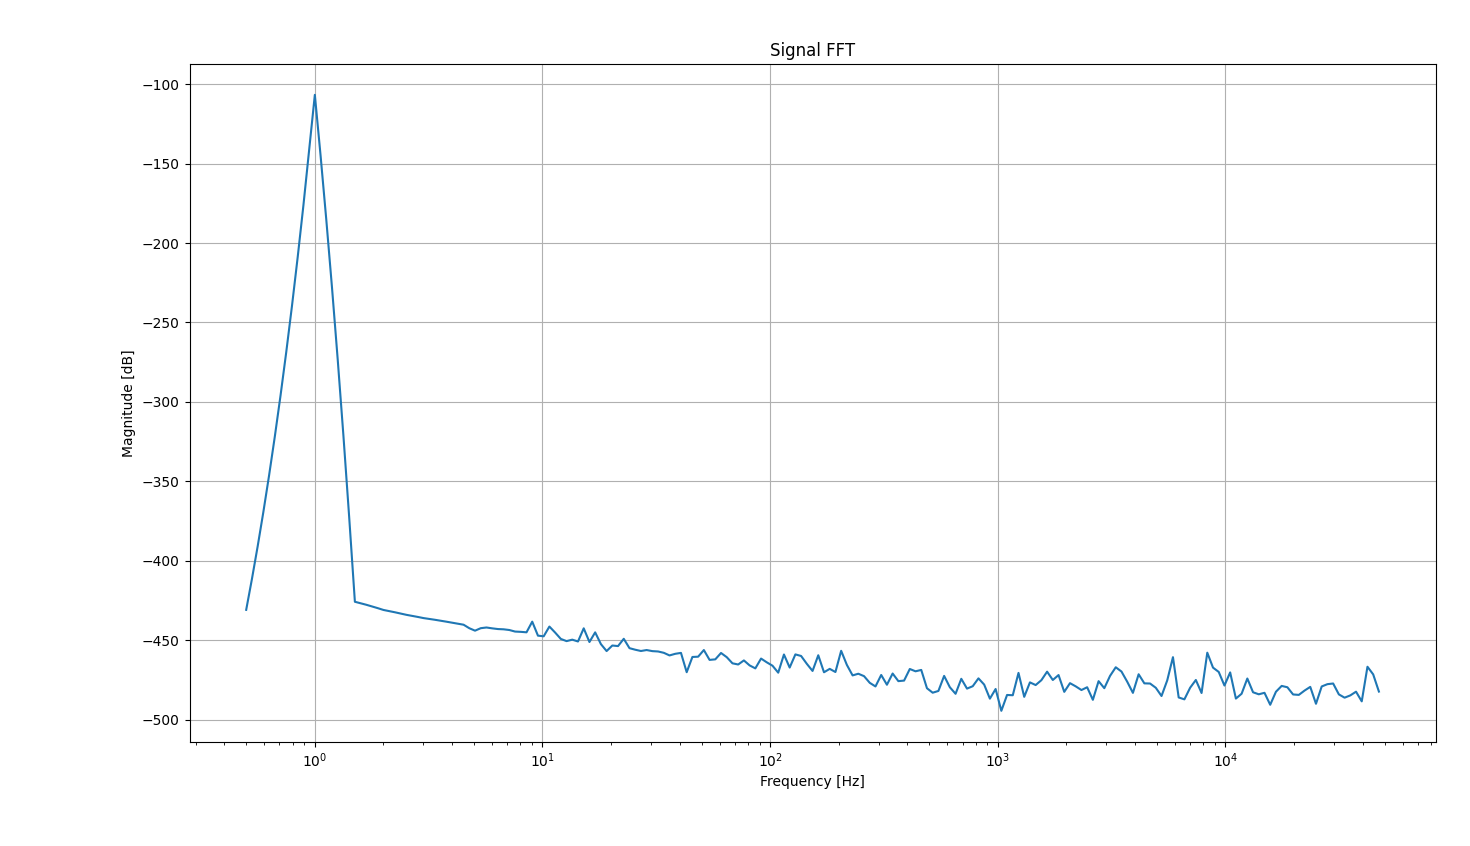
\includegraphics[width=\textwidth]{Images/Vin_ideal.png}
        \caption{$V_{IN}(f)$ - Fourier Transform of $v_{in}(t)$.}
        \label{fig:Vin_freq_ideal}
    \end{subfigure}

    \begin{subfigure}[b]{0.4\textwidth}
        \centering
        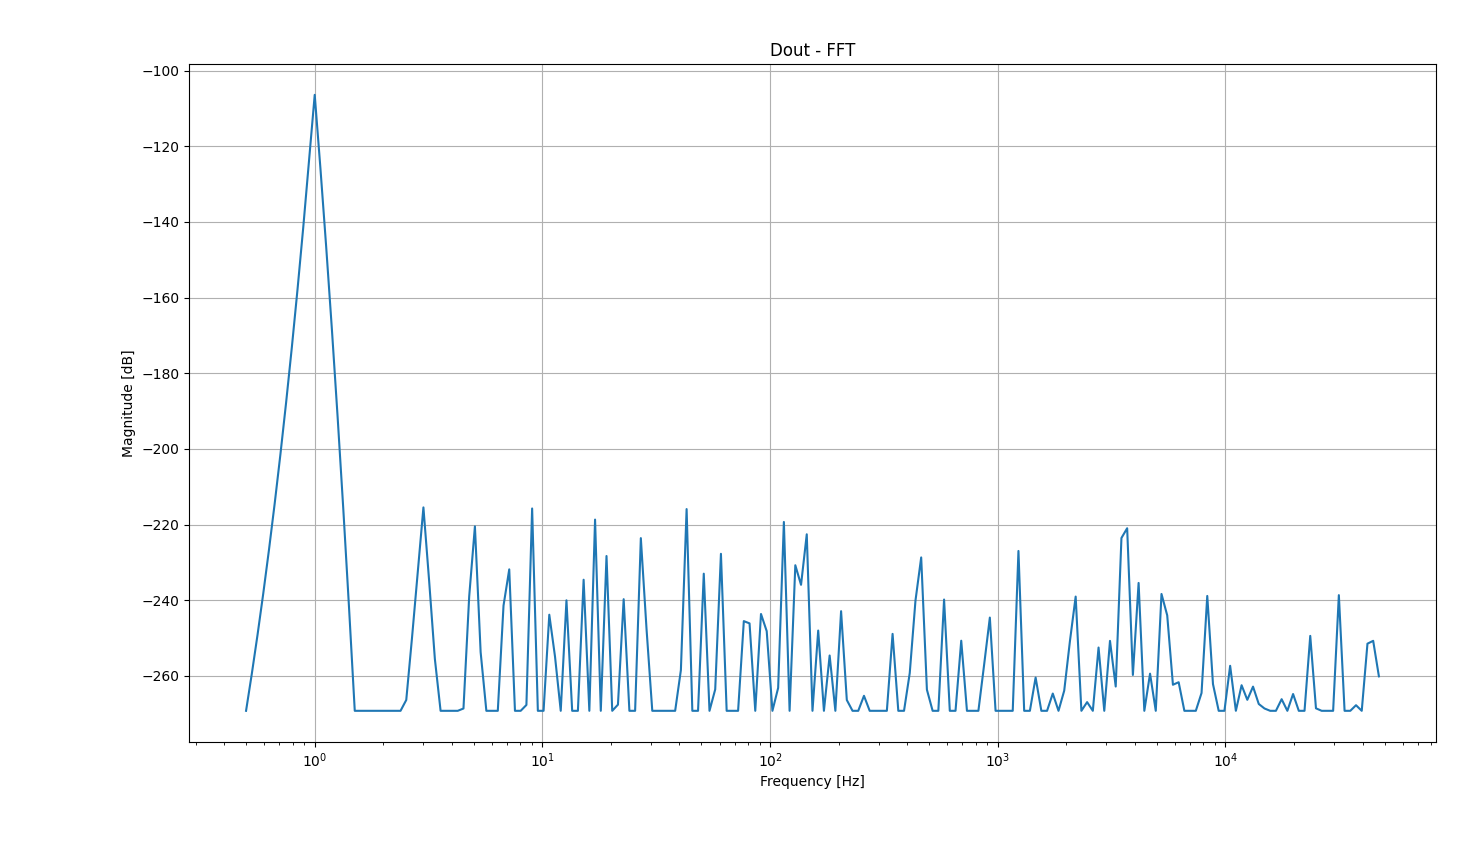
\includegraphics[width=\textwidth]{Images/Dout_ideal.png}
        \caption{$V_{OUT}(f)$ - Fourier Transform $v_{out}(t)$.} 
        \label{fig:Vout_freq_ideal}
    \end{subfigure}%
    \begin{subfigure}[b]{0.4\textwidth}
        \centering
        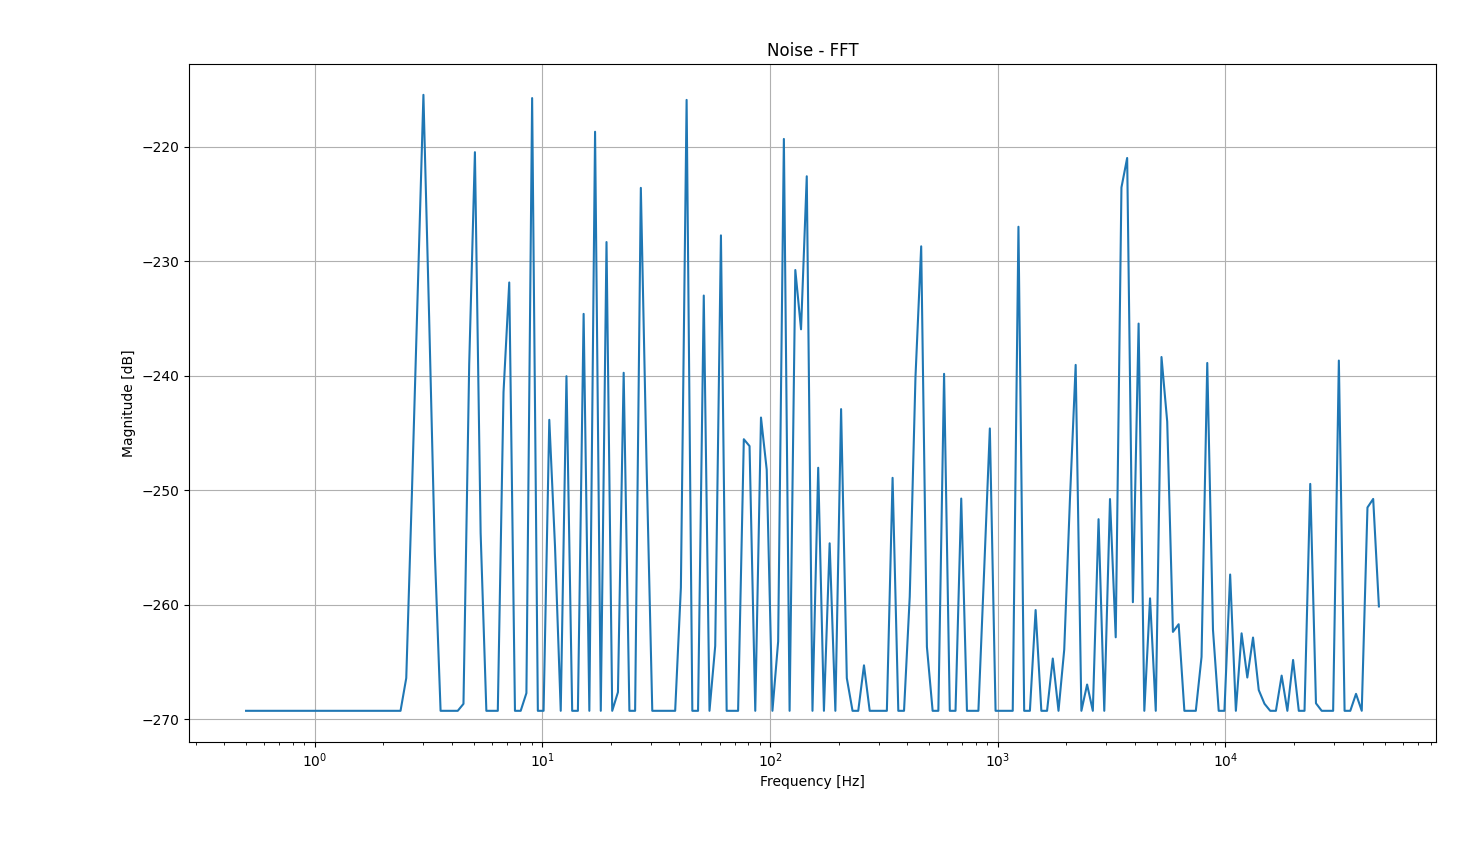
\includegraphics[width=\textwidth]{Images/Noise_Ideal.png}
        \caption{$N(f)$ - Noise Spectrum.}
        \label{fig:Noise_freq_ideal}
    \end{subfigure}

    \caption{Noise spectrum for ideal ADC.}
    \label{fig:Noise Ideal}
\end{figure}

When implementing this, it is important to remember that code operates in discrete time, which has specific effects.  To avoid spectral leakage, the sample length was chosen such that the input sine completes an integer number of periods. According to the Nyquist theorem, the maximum frequency that can be represented is $F_s/2$, therefore the integral ends at $F_s/2$ and not $+\infty$. By using a high sampling rate and a low input frequency, the noise introduced during sampling becomes negligible.

\subsubsection{Code Validation}

To validate the code, this was tested for the ideal ADC, Equation \ref{eq:IdealSNR} shows the ideal $SNR$ value for a ADC. 

\begin{equation}
    SNR_{MAX} = 6.02\cdot n+1.76~~[\si{\decibel}] \textsuperscript{\cite{analogIntegratedCircBook}}
    \label{eq:IdealSNR}
\end{equation}

Which for a 12 bit ADC gives an ideal $SNR$ of $74~~\si{\decibel}$. The calculated value through the python scripts gives an $SNR = 73.9761~\si{\decibel}$, validating the implementation.



% \textcolor{red}{Using the previous expression, write a Matlab/Octave model of the behavior of
% this SAR ADC, including the offset error of the comparator. Note that the SAR
% ADC uses two capacitor arrays (split into LSB and MSB arrays) and fully
% differential signals. Include random errors into the capacitors' values and into
% the comparator's offset voltage.}

% \textcolor{red}{Carefully explain all the relevant parts of your code, including how you obtained the values for the capacitors in the arrays.}

% \textcolor{red}{Demonstrate that your code is working correctly, by first presenting the INL and DNL for the case of zero errors in the circuit. Also present the evolution of Vxp and Vxn for each step for a given input voltage.}